\documentclass[12pt,a4paper]{article}
\usepackage[utf8]{inputenc}
\usepackage{amsmath}
\usepackage{amsfonts}
\usepackage{amssymb}
\usepackage{graphicx}
\usepackage[utf8]{inputenc}
\usepackage[T1]{fontenc}
\usepackage{CJKutf8}
\usepackage[english,russian]{babel}
\graphicspath{{graphs/}}
\author{Будакян Ян}
\title{Статистический анализ спектра акустического сигнала электромеханического устройства}
\begin{document}

\begin{titlepage}
\begin{center}
{\small\textsc{Московский Государственный Университет им. М.\,В. Ломоносова}}
\vskip 1pt \hrule \vskip 3pt
{\small\textsc{Физический факультет}}
\vfill
{\Large Курсовая работа\vskip 12pt\bfseries Статистический анализ спектра акустического сигнала \space электромеханического устройства}	
\end{center}
\vfill
\begin{flushright}
{Выполнил студент 212 группы \\Будакян Я.\,С.\vskip 12pt Научный руководитель \\к.т.н. доц. Грачев Е.\,А.}
\end{flushright}
\vfill
\begin{center}
Москва, 2015
\end{center}
\end{titlepage}

\tableofcontents
\newpage

\section{Введение}

Различные акустические сигналы несут в себе огромное множество разнообразной информации. Задачи анализа акустических сигналов возникают не только при проведении большого количества разных физических экспериментов, но и в сугубо прикладных целях.

Одной из таких задач является задача о разладке(или, как обобщение, "переключения состояний"\space --- сегментации) сигнала. Например, мы снимаем некоторый сигнал с какого-либо объекта. В какой-то момент с объектом что-то происходит, и свойства сигнала некоторым образом меняются. Задача состоит в том, чтобы автоматически отслеживать такие моменты, и принимать в зависимости от этого какие-либо решения. Практические приложения этой задачи довольно разнообразны. Они возникают в различных областях:
\begin{itemize}
\item Обнаружение неисправностей и диагностика
\item Техническое обслуживание промышленности
\item Безопасность сложных систем(самолетов, лодок, ракет, АЭС, и т.д.)
\item Контроль качества
\item Прогнозирование природных катастроф(землетрясения, цунами, и т.д.)
\item Мониторинг в биомедицине 
\end{itemize}

В качестве математической модели таких акустических сигналов будет использоваться авторегрессионный процесс. Такой подход часто применяется при моделировании различных случайных сигналов, от человеческой речи и шума от устройств \cite{TVAR, vehicles} до биологических сигналов \cite{bio}.

\section{Постановка задачи}
Дан авторегрессионный процесс
$$x_t = \phi_0(h_t) + \sum_{i=1}^{n} \phi_i(h_t)x_{t-i} + B(h_t)\xi_t$$

где $\xi_t$ - стандартный белый шум.\\
Параметры процесса могут скачкообразно изменяться, принимая в каждый момент времени $t\geq 0$ один  из $m$ известных наборов значений\\ $\phi_0(h_t),\dots,\phi_n(h_t), B(h_t),;h_t \in \{1,\dots,m\}$.
Также задана матрица $Q$ вероятностей переходов между наборами параметров(классами):
$$P(h_t|h_{t-1}) = q(h_{t-1}, h_t)$$

Под задачей сегментации понимается задача отношения каждого отсчета процесса $x_t$ некоторому классу $h_t$, т.е. восстановление ненаблюдаемой последовательности "переключений"\space состояний $h_i \longrightarrow h_j$.

Одним из алгоритмов, решающим задачу сегментации является алгоритм на основе метода динамического программирования~\cite{burobin}.

\section{Алгоритм сегментации на основе метода\\ динамического программирования}
При данном подходе оптимальной считается сегментация $H_1^N$(набор чисел $h_t$, соответствующих отсчетам $x_t$), доставляющая минимум критерию
\begin{equation}
\label{criteria}
J(H_0^N) = d_0(h_0) +\sum_{t=1}^{N}\beta_t(h_{t-1},h_t)
\end{equation}
$$\beta_t(h_{t-1},h_t) = \frac{1}{2B(h_t)}[x_t-\phi_0(h_t)-\sum_{i=1}^{n}\phi_i(h_t)x_{t-i}]^2-\ln q(h_{t-1},h_t)$$

В критерии (\ref{criteria}) величина $\beta_t(h_{t-1},h_t)$ имеет смысл несогласованности формы кривой в точке $t$ при данной предыстории $X_{t-n}^{t-1}$ с предполагаемыми значениями параметров авторегрессии с учетом априорной предпочтительности данных значений, учитываемой членом $\ln q(h_{t-1},h_t)$;\\$d_0(h_0)$ - член, выражающий априорную нежелательность отнесения нулевого отсчета классу $h_0 = 1,\dots,m$.
Определим последовательность векторов
$$d_t(h_t) = \underset{H_0^{t-1}}{min}[d_0(h_0) +\sum_{s=1}^{t-1} \beta_s(h_{s-1},h_s) + \beta_t(h_{t_1},h_t)],\;h_t = 1,\dots,m;\;t = 1,\dots,N$$
Компоненты этого вектора показывают, какое минимальное значение критерия (\ref{criteria}) можно получить за счет различной классификации отсчетов до $(t-1)$-го включительно, если принять класс последнего отсчета равным $h_t$. Поскольку минимальная компонента вектора $d_N(h_N)$ совпадает с минимальным значением критерия (\ref{criteria}), то 
\begin{equation}
\label{cond_for_hN}
\hat{h}_N = \arg\min[d_N(h_N)]
\end{equation}
является последним элементом оптимальной 
сегментации $\hat{H}_0^N$.\\
Векторы $d_t(h_t)$ вычисляются рекуррентно по правилу
$$d_t(h_t) = \min[d_{t-1}(h_{t-1})+\beta_t(h_{t-1},h_t)],$$
начиная с начальных значений $d_0(h_0) = -\ln p(h_0)$.
При этом в процессе вычисления векторов $d_t(h_t)$ величины
$$k_t(h_t) = \arg\min[d_{t-1}(h_{t-1})+\beta_t(h_{t-1},h_t)]$$
записываются в матрицу $K_1^N[m \times N]$. Эта матрица позволяет найти оптимальную последовательность $\hat{H}_0^{N-1}$ по рекуррентной формуле
\begin{equation}
\label{rule_9}
\hat{h}_{s-1} = k_s(\hat{h}_s),\; s = N, N-1, \dots, 1
\end{equation}
с начальным условием (\ref{cond_for_hN}).

Описанный алгоритм позволяет найти оптимальную сегментацию, но он работает в "оффлайн"\space режиме, т.е. анализ проводится уже после того, как весь сигнал получен. Однако, этот подход можно обобщить и на случай "онлайн"\space сегментации, т.е. анализа сразу во время считывания сигнала.\\

Возьмем от построенной матрицы $K_1^N$ часть $K_1^t$ для некоторого момента времени t. Она позволяет найти оптимальную сегментацию $\tilde{H}_0^{t-1}$, при начальном условии
\begin{equation}
\label{vect_11}
\tilde{h}_t^i = i,\; i=1,\dots,m.
\end{equation}
Можно ожидать, что при достаточно больших $t$ найдется момент времени $u_t<t$ такой, что на интервале $0\leq s \leq u_t$ выполнится условие
\begin{equation}
\label{cond_12}
\tilde{h}_s^1 = \dots = \tilde{h}_s^m.
\end{equation}
Выполнение этого условия означает, что совпадут все построенные сегментации $\tilde{H}_0^{u_t}$ при различных выборах $\tilde{h}_t$. В таком случае, этот кусок сегментации будет содержаться в оптимальной сегментации всего сигнала как составная часть и может быть построен, не дожидаясь последнего отсчета.\\

Назовем $u_t$ правой границей принятия решения --- это номер последнего отсчета сигнала, для которого уже принято решение о его принадлежности некоторому классу. Для нулевого отсчета полагается $u_0 = -1.$ Также, назовем особыми моментами времени $t^*$ моменты, в которые меняется граница принятия решения, первый особый момент $t^* = 0.$\\ Таким образом, работа алгоритма будет заключаться в проверке, является ли текущий момент времени особым, на каждом шаге вычислений, и, в случае особого момента, построении куска оптимальной сегментации.\\

Пусть $t^*$ последний зафиксированный особый момент времени, с соответствующей границей $u_{t^*}$. Начиная с $t = t^* +1$ на каждом шаге вычисляется новый столбец $k_t(i),\; i = 1,\dots,m$ по правилу
$$k_t(i) = \arg\min[d_{t-1}(j)+\beta_t(j,i)],$$
добавляемый к матрице $K_{u_t+2}^{t-1}$. Для обнаружения особого момента рекуррентно пересчитывается вектор $g_t(i),\; i =1,\dots,m$ по правилу
$$g_t(i) = g_{t-1}[k_t(i)]$$ с начальным условием
$$g_{t^*}(i) = \tilde{h}_{u_{t^*}+1}^i$$
Компоненты этого вектора показывают, к какому классу будет отнесен отсчет с номером $u_t + 1$, если зафиксировать принадлежность отсчета $\tilde{h}_t=i.$\\
Пока не выполняется равенство
\begin{equation}
\label{cond_16}
g_t(1) = \dots = g_t(m)
\end{equation}
особый момент еще не наступил, положение границы принятия решения не изменяется и происходит накопление матрицы $K.$ Момент выполнения условия (\ref{cond_16}) регистрируется как очередной особый момент $t^*$. Для того, чтобы найти новую границу принятия решения $u_{t^*}$ нужно, приняв в качестве начального условия вектор (\ref{vect_11}), вычислять в обратном порядке $s = t-1, t-2,\dots$ векторы $\tilde{h}_s^i,\; i = 1,\dots, m$, пока на некотором шаге $s^*$ выполнится условие (\ref{cond_12}). Тогда $u_{t^*} = s^*$, и можно строить отрезок оптимальной сегментации между предыдущим и новыми положениями границы принятия решений по рекуррентному правилу (\ref{rule_9}). Фрагмент матрицы $K_{u_{t^*-1}+2}^{u_{t^*}+1}$ более не нужен и может быть сброшен.

%\\Дописать....

\section{Алгоритм CUSUM}
Другой алгоритм для решения той же задачи --- это алгоритм на основе статистики кумулятивных сумм. \\
Рассмотрим последовательность распределений случайных величин $x_t$ при условии фиксированной предыстории $x_{t-1},\dots,x_1$. Поскольку распределение до и после момента переключения отличается только коэффициентами авторегрессии $\phi_k(h_t)$, то условное распределение величин $x_t$ $p(x_t|x_{t-1},\dots,x_1)$ до и после момента переключения отличается математическим ожиданием; отличием дисперсии шума можно пренебречь. Будем также считать, что распределение $x_t$ является нормальным. Зафиксируем некоторый переход $h_i \longrightarrow h_j$ и вычислим плотности распределения $p_i(x_t|x_{t-1},\dots,x_1)$ и $p_j(x_t|x_{t-1},\dots,x_1)$ в каждой точке исходного ряда $x_t$. Найдем логарифм отношения правдоподобия
$$L_t = \ln \frac{p_j(x_t|x_{t-1},\dots,x_1)}{p_i(x_t|x_{t-1},\dots,x_1)}$$
Если $L_t > 1$, то вероятность, что отсчет $x_t$ был получен из распределения, соответствующего классу $h_j$, выше, чем обратного.\\
Найдем $L_t$ в явном виде:
$$p_i(x_t|x_{t-1},\dots,x_1) = \frac{1}{\sqrt{2\pi\sigma^2(h_i)}} \exp\bigg\{-\frac{1}{2\sigma^2(h_i)}(x_t - \phi_0(h_i) -\sum_{k=1}^{n} \phi_k(h_i) x_{t-k})^2\bigg\},$$
$$p_j(x_t|x_{t-1},\dots,x_1) = \frac{1}{\sqrt{2\pi\sigma^2(h_j)}} \exp\bigg\{-\frac{1}{2\sigma^2(h_j)}(x_t - \phi_0(h_j) -\sum_{k=1}^{n} \phi_k(h_j) x_{t-k})^2\bigg\}$$
Поскольку мы считаем, что дисперсия при переключении не меняется, т.е. $\sigma^2(h_i) = \sigma^2(h_j)$, то:

$$L_t = \ln \frac{p_j(x_t|x_{t-1},\dots,x_1)}{p_i(x_t|x_{t-1},\dots,x_1)} = $$
$$= \ln \frac{\frac{1}{\sqrt{2\pi\sigma^2(h_j)}} \exp\big\{-\frac{1}{2\sigma^2(h_j)}(x_t - \phi_0(h_j) -\sum_{k=1}^{n} \phi_k(h_j) x_{t-k})^2\big\}}{\frac{1}{\sqrt{2\pi\sigma^2(h_i)}} \exp\big\{-\frac{1}{2\sigma^2(h_i)}(x_t - \phi_0(h_i) -\sum_{k=1}^{n} \phi_k(h_i) x_{t-k})^2\big\}} =$$
$$= \ln \frac{\exp\{-(x_t - \phi_0(h_j) -\sum_{k=1}^{n} \phi_k(h_j) x_{t-k})^2\}}{\exp\{-(x_t - \phi_0(h_i) -\sum_{k=1}^{n} \phi_k(h_i) x_{t-k})^2\}} = $$
$$= (x_t - \phi_0(h_i) -\sum_{k=1}^{n} \phi_k(h_i) x_{t-k})^2 - (x_t - \phi_0(h_j) -\sum_{k=1}^{n} \phi_k(h_j) x_{t-k})^2$$
Кумулятивные суммы рассчитываются с помощью рекуррентных соотношений:
\[
\left\{
\begin{aligned}
&z_1 = 0, \\
&z_t = \max(0, z_{t-1} + L_t), \;t = 2,3,\dots \\
\end{aligned}
\right.
\]
Теперь необходимо задать некоторый порог $T_{ij}$. Если на некотором шаге вычислений $t$ значение $z_t$ превысило $T_{ij}$, то считается, что произошло переключение $h_i \longrightarrow h_j$.\\
Таким образом, работа алгоритма представляет собой вычисление $m(m-1)$ кумулятивных сумм до обнаружения первого момента переключения и $m-1$ на каждом последующем шаге(так как переключения происходят последовательно).

\section{Результаты}
Оба описанных выше алгоритма были реализованы в программном коде на языке Python. Было проведено экспериментальное исследование алгоритмов на модельном сигнале и на реальных данных с электромеханического устройства - вентилятора.
\subsection{Модельный сигнал}
Ниже приведены графики(\ref{signal_1_burobin}, \ref{signal_1_cusum}, \ref{signal_2_burobin}, \ref{signal_2_cusum}), на которых изображены сегментации модельного сигнала, построенные обеими программами, наложенные на оригинальную сегментацию.\\
\begin{figure}[h]
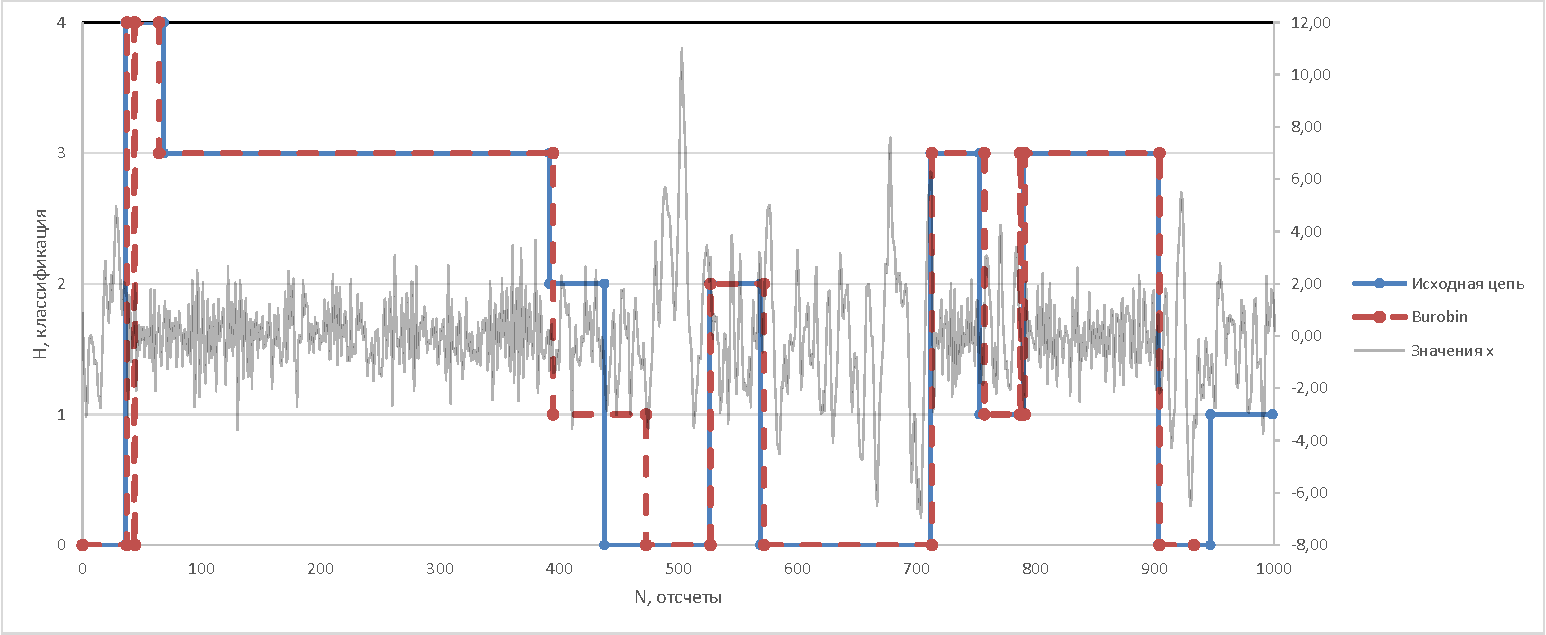
\includegraphics[width=\linewidth]{1k_burobin}
\caption{Сигнал 1, t = 1000, алгоритм\cite{burobin}}
\label{signal_1_burobin}
\end{figure}
\begin{figure}[h]
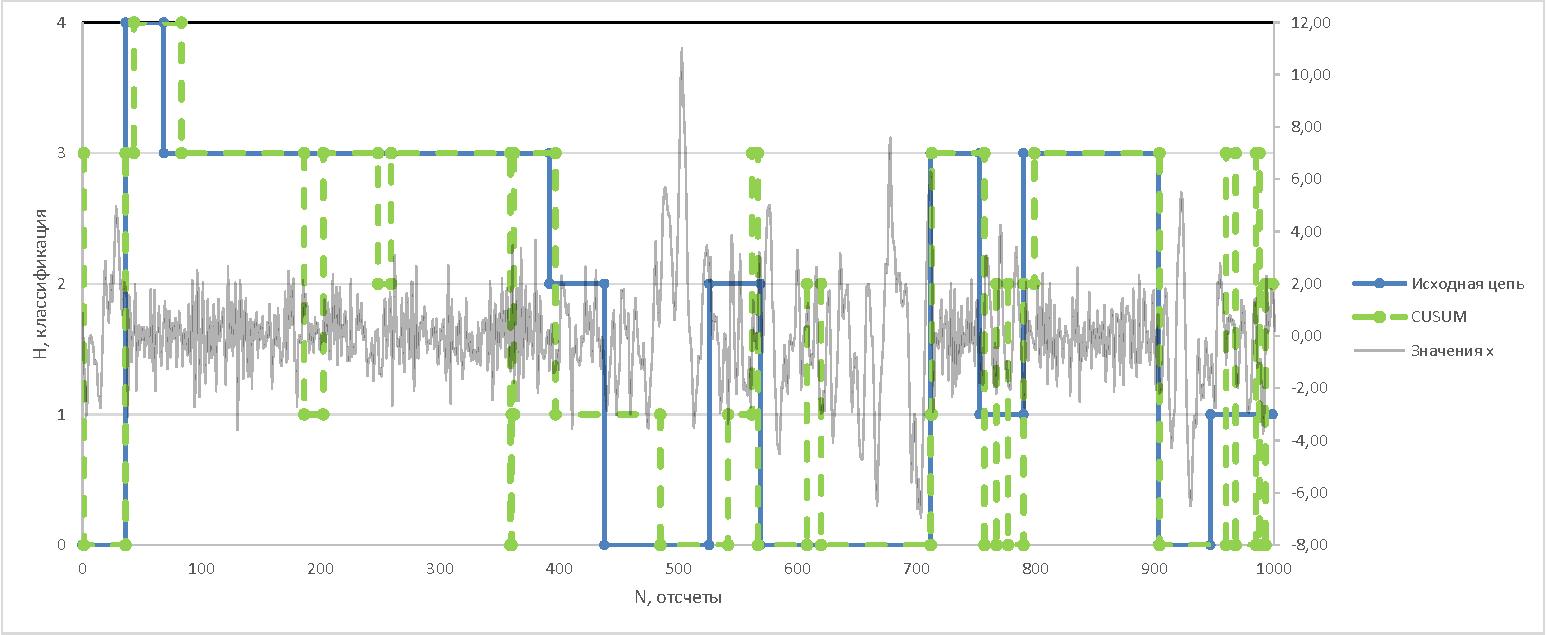
\includegraphics[width=\linewidth]{1k_cusum}
\caption{Сигнал 1, t = 1000, алгоритм CUSUM}
\label{signal_1_cusum}
\end{figure}
\begin{figure}[h]
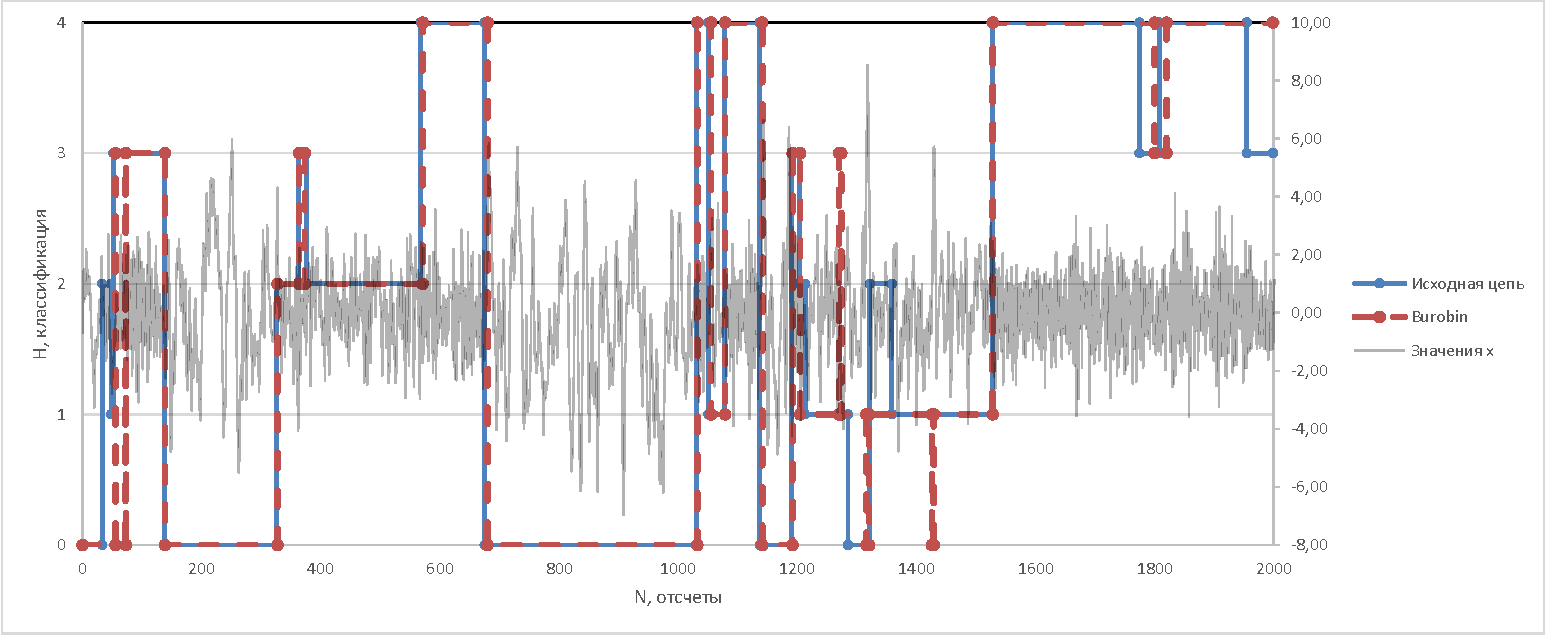
\includegraphics[width=\linewidth]{2k_burobin}
\caption{Сигнал 2, t = 2000, алгоритм\cite{burobin}}
\label{signal_2_burobin}
\end{figure}
\begin{figure}[h]
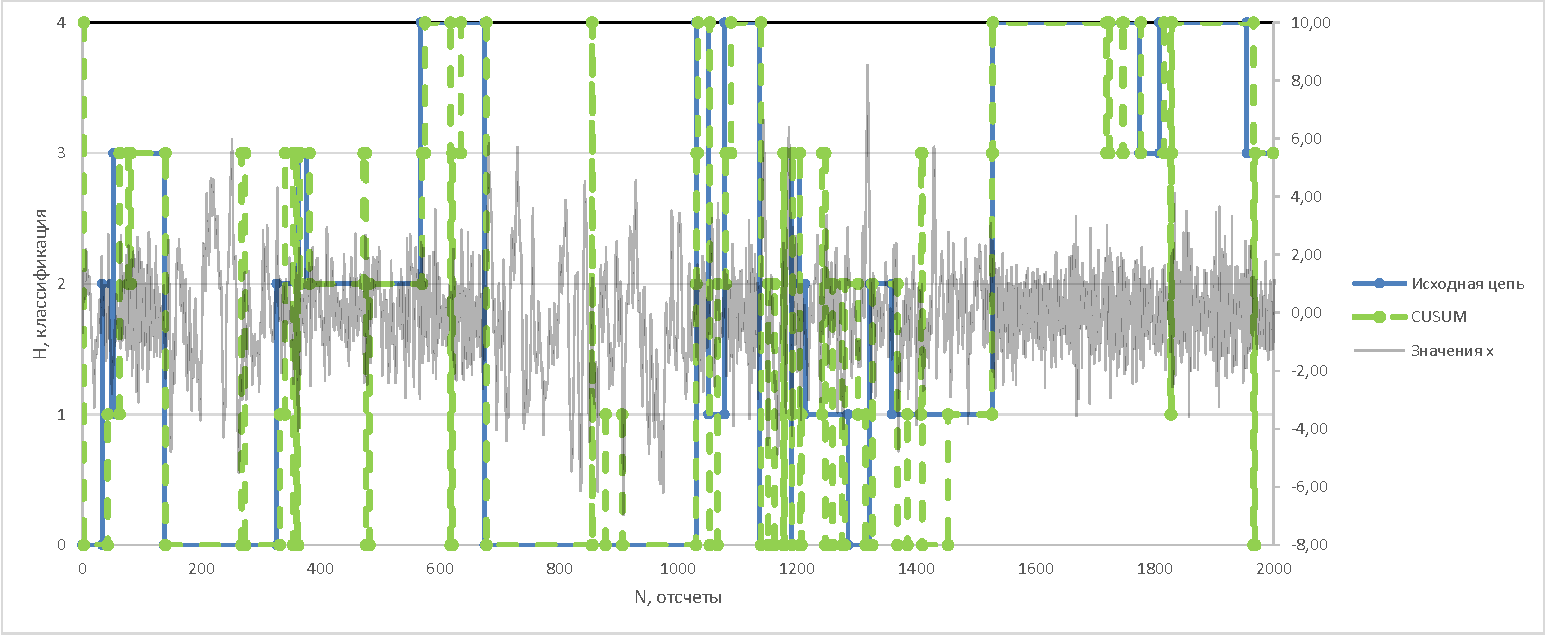
\includegraphics[width=\linewidth]{2k_cusum}
\caption{Сигнал 2, t = 2000, алгоритм CUSUM}
\label{signal_2_cusum}
\end{figure}

Было проведено исследование качества обоих алгоритмов. В качестве меры точности алгоритма было взято среднее время совпадения построенной сегментации с оригинальной, усредненное по всем запускам:
$$Q_A = \frac{1}{N}\sum_{i=1}^{N}\bigg[\frac{1}{T}\sum_{t=1}^{T}\delta_i(h_t^A,h_t^0)\bigg],$$
где
$$\begin{matrix}
\delta_i(h_t^A,h_t^0) & = & \left\{
\begin{matrix}
0, & \mbox{если } h_t^A \neq h_t^0 \\
1, & \mbox{если } h_t^A = h_t^0 
\end{matrix}\right.
\end{matrix}
$$
в $i-$том запуске, а $h_t^A \mbox{ и } h_t^0$ есть классификации отсчета $x_t$ по версии алгоритма $A$ и истинное значение соответственно.\\
Для экспериментов использовался генератор модельного сигнала с \\$n = 2, m = 5$. Параметры модельного сигнала указаны в таблице \ref{signal_param}.
\\

\begin{table}[h]
\caption{Параметры модельного сигнала}
\label{signal_param}
\begin{center}
\begin{tabular}{|c|c|c|c|c|}
\hline
h & $\phi_0$ & $\phi_1$ & $\phi_2$ & $B$\\
\hline
0 & 0 & 1.36 & -0.49 & 1\\
\hline
1 & 0 & 1.02 & -0.40 & 1\\
\hline
2 & 0 & 0.82 & -0.49 & 1\\
\hline
3 & 0 & 0 & -0.49 & 1\\
\hline
4 & 0 & -0.82 & -0.49 & 1\\
\hline
\multicolumn{5}{|c|}{$q_{ii} = 0.99$}\\
\hline
\multicolumn{5}{|c|}{$q_{ij} = 0.0025$, $i \neq j$}\\
\hline
\end{tabular}
\end{center}
\end{table}
Усреднение проводилось по $N = 20000$ запусков. Были получены следующие результаты:
$$t = 1000,\; Q_B = 0.86795,\; Q_{CUSUM} = 0.76240$$
$$t = 2000,\; Q_B = 0.86408,\; Q_{CUSUM} = 0.75599$$
$$t = 3000,\; Q_B = 0.86235,\; Q_{CUSUM} = 0.75323$$

\subsection{Сигнал с вентилятора}

Были произведены записи шума вентилятора в нормальном режиме работы и с разладкой - в работающий вентилятор засовывалась бумажка. Формат записи - 20 секунд нормального режима, 20 секунд - разладка, последние 20 секунд - опять нормальный режим. Частота дискретизации записи - 44100 Гц. Всего было сделано 3 записи по 1 минуте.
После было составлено 3 обрезанных до 3-х секунд сигналов для анализа(по одной вырезанной секунде из каждого 20-секундного отрезка). Общее количество отсчетов в каждом сигнале составило $3$с $\cdot\;44100$Гц $ = 132300.$

Один из сигналов был использован для подбора параметров для алгоритмов. С помощью МНК были определены коэффициенты авторегрессии с глубиной модели $P = 10$. На рисунке \ref{autoregr_params} показаны зависимости коэффициентов авторегрессии для этого сигнала а) до разладки, б) во время разладки от количества отсчетов, анализируемых МНК.
\begin{figure}[h]
\begin{minipage}[h]{0.49\linewidth}
\center{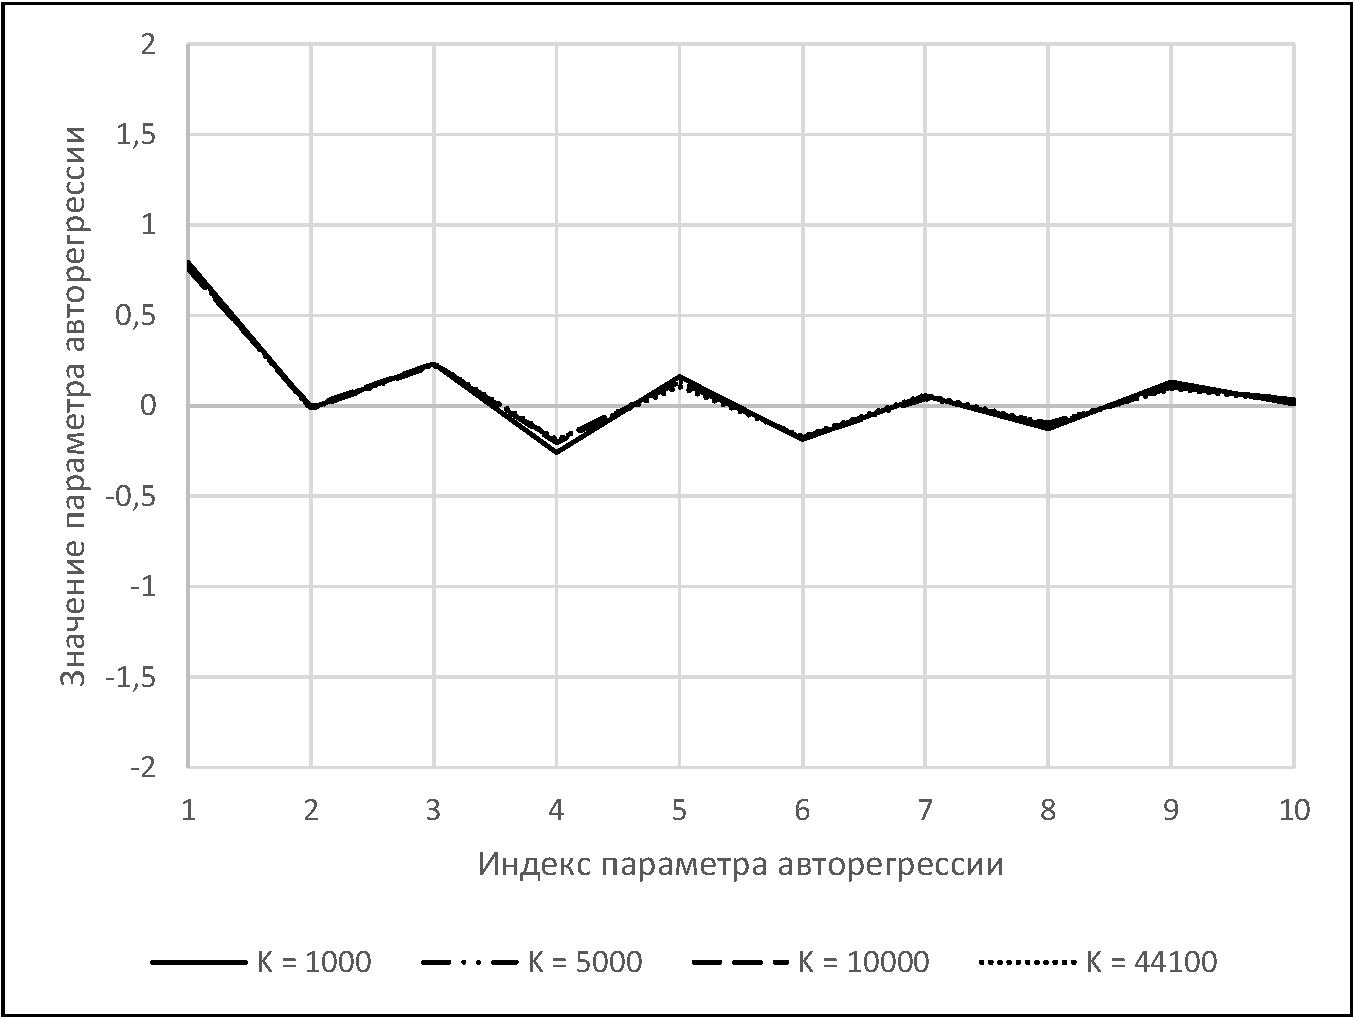
\includegraphics[width=\linewidth]{autoregression_params_normal} \\а)}
\end{minipage}
\begin{minipage}[h]{0.49\linewidth}
\center{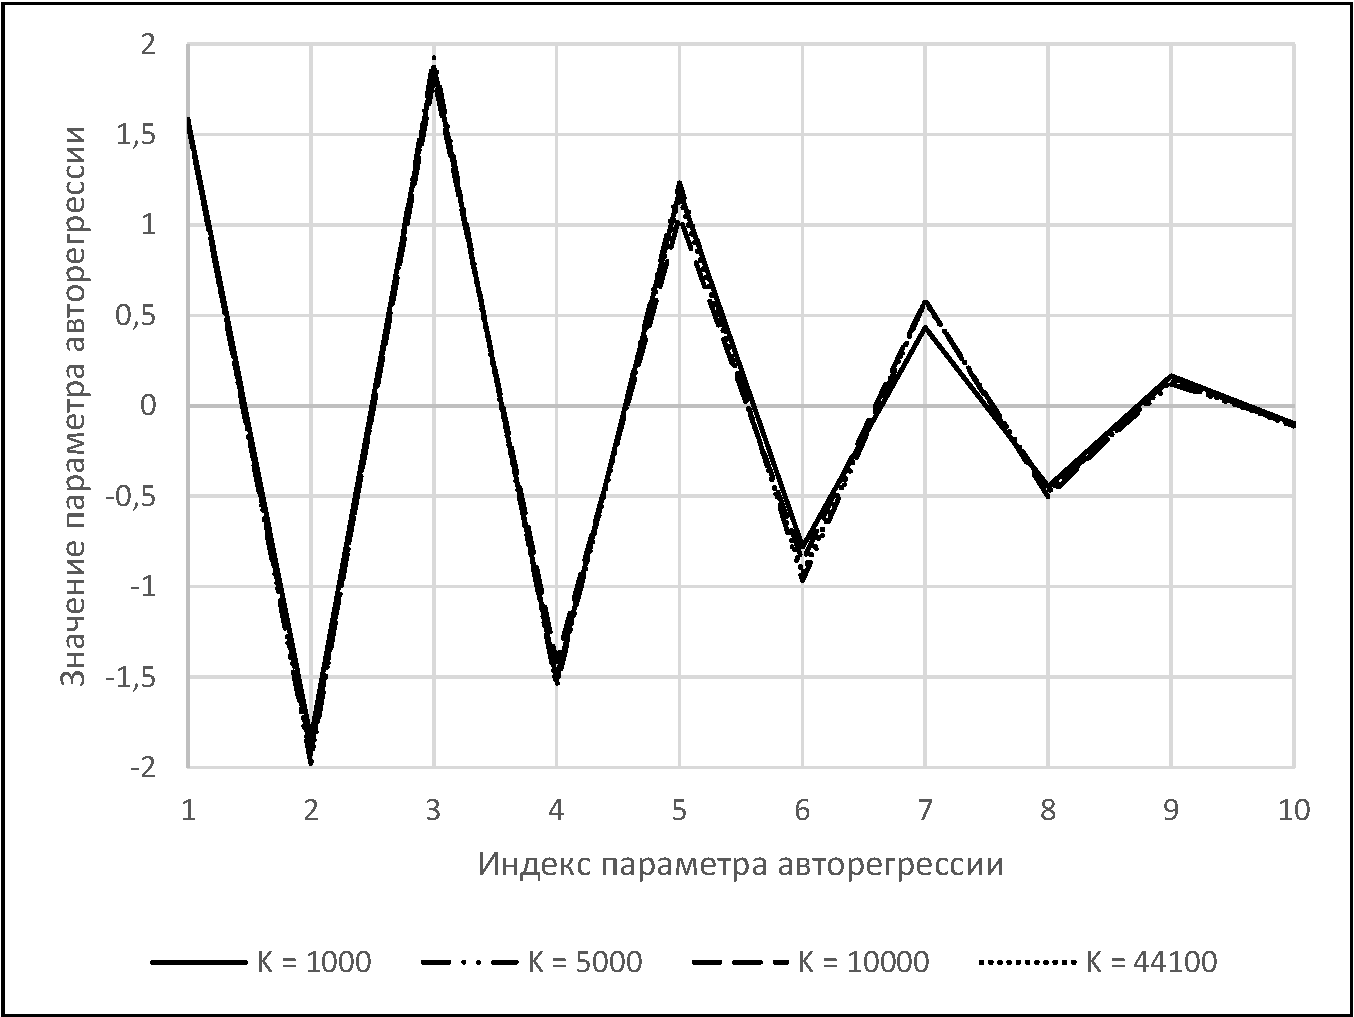
\includegraphics[width=\linewidth]{autoregression_params_disaster} \\ б)}
\end{minipage}
\caption{Значения коэффициентов авторегрессии до и во время разладки}
\label{autoregr_params}
\end{figure}
Оценки параметров авторегрессий приведены в таблице \ref{AR_params_table}.
\begin{table}[h]
\caption{Оценки коэффициентов авторегрессий, полученные МНК}
\label{AR_params_table}
\begin{tabular}{|c|c|c|c|c|c|c|c|c|c|c|c|c|}
\hline
h & $\phi_0$ & $\phi_1$ & $\phi_2$ & $\phi_3$ & $\phi_4$ & $\phi_5$ & $\phi_6$ & $\phi_7$ & $\phi_8$ & $\phi_9$ & $\phi_{10}$\\
\hline
0 & 0 & 0.78 & 0 & 0.23 & -0.19 & 0.11 & -0.17 & 0.06 & -0.1 & 0.1 & 0\\
\hline
1 & 0 & 1.58 & -1.94 & 1.88 & -1.53 & 1.16 & -0.93 & 0.58 & -0.47 & 0.14 & -0.11\\
\hline
\end{tabular}
\end{table}

В таблице \ref{AR_params_table} $h_0$ соответствует нормальной работе вентилятора, а $h_1$ - разладке. Подобранные параметры для алгоритма\cite{burobin} и CUSUM составили $B(h_i) = 10^5,\; q_{ii} = 0.99999,\; T_{ij} = 4 \cdot 10^6.$ Полученные обоими алгоритмами сегментации изображены на рисунке \ref{cropped_1}(вариант а) соответствует алгоритму\cite{burobin}, б) - CUSUM)
\begin{figure}[h]
\begin{minipage}[h]{0.49\linewidth}
\center{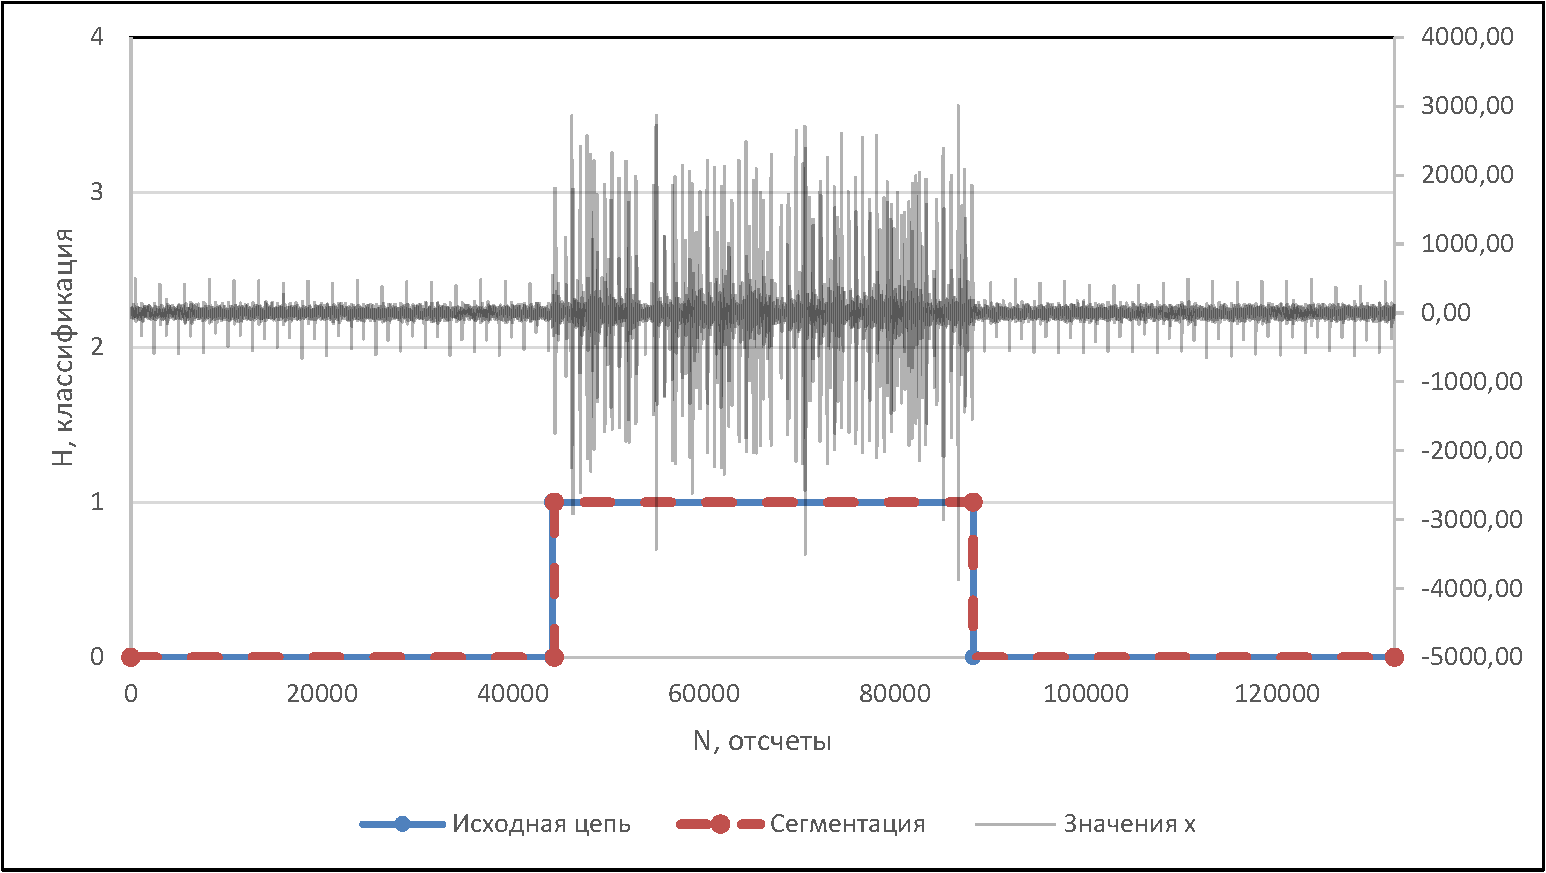
\includegraphics[width=\linewidth]{signal_cropped_1_burobin} \\а)}
\end{minipage}
\begin{minipage}[h]{0.49\linewidth}
\center{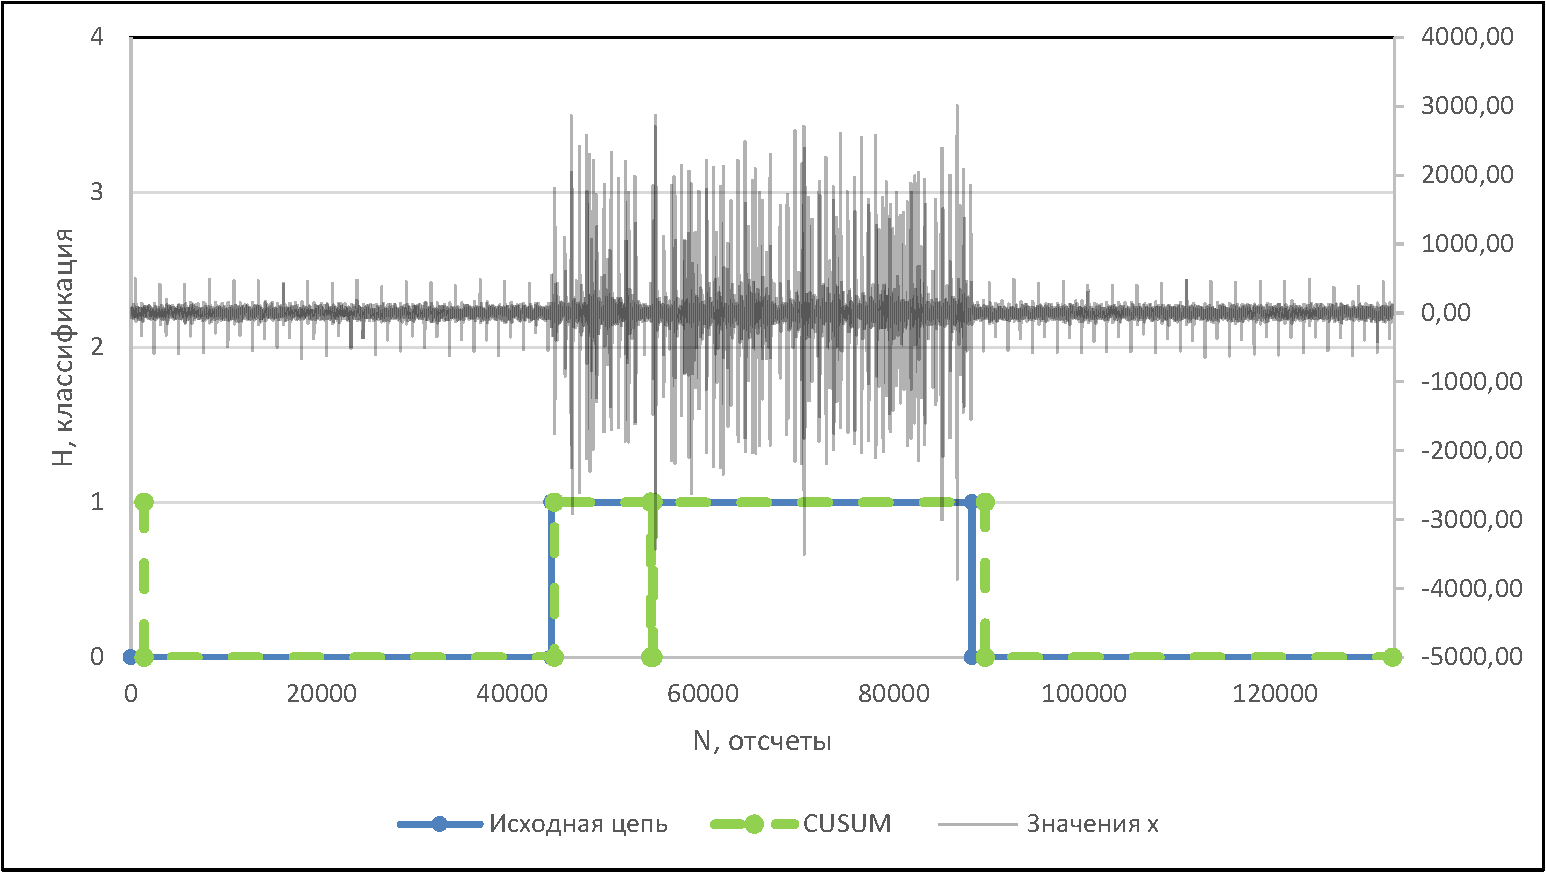
\includegraphics[width=\linewidth]{signal_cropped_1_cusum} \\б)}
\end{minipage}
\caption{Сегментация первого сигнала с вентилятора обоими алгоритмами}
\label{cropped_1}
\end{figure}

Потом, не изменяя найденных параметров, алгоритмы были применены к другим двум оставшимся сигналам. Результаты изображены на графиках \ref{cropped_2} и \ref{cropped_3}.

\begin{figure}[h]
\begin{minipage}[h]{0.49\linewidth}
\center{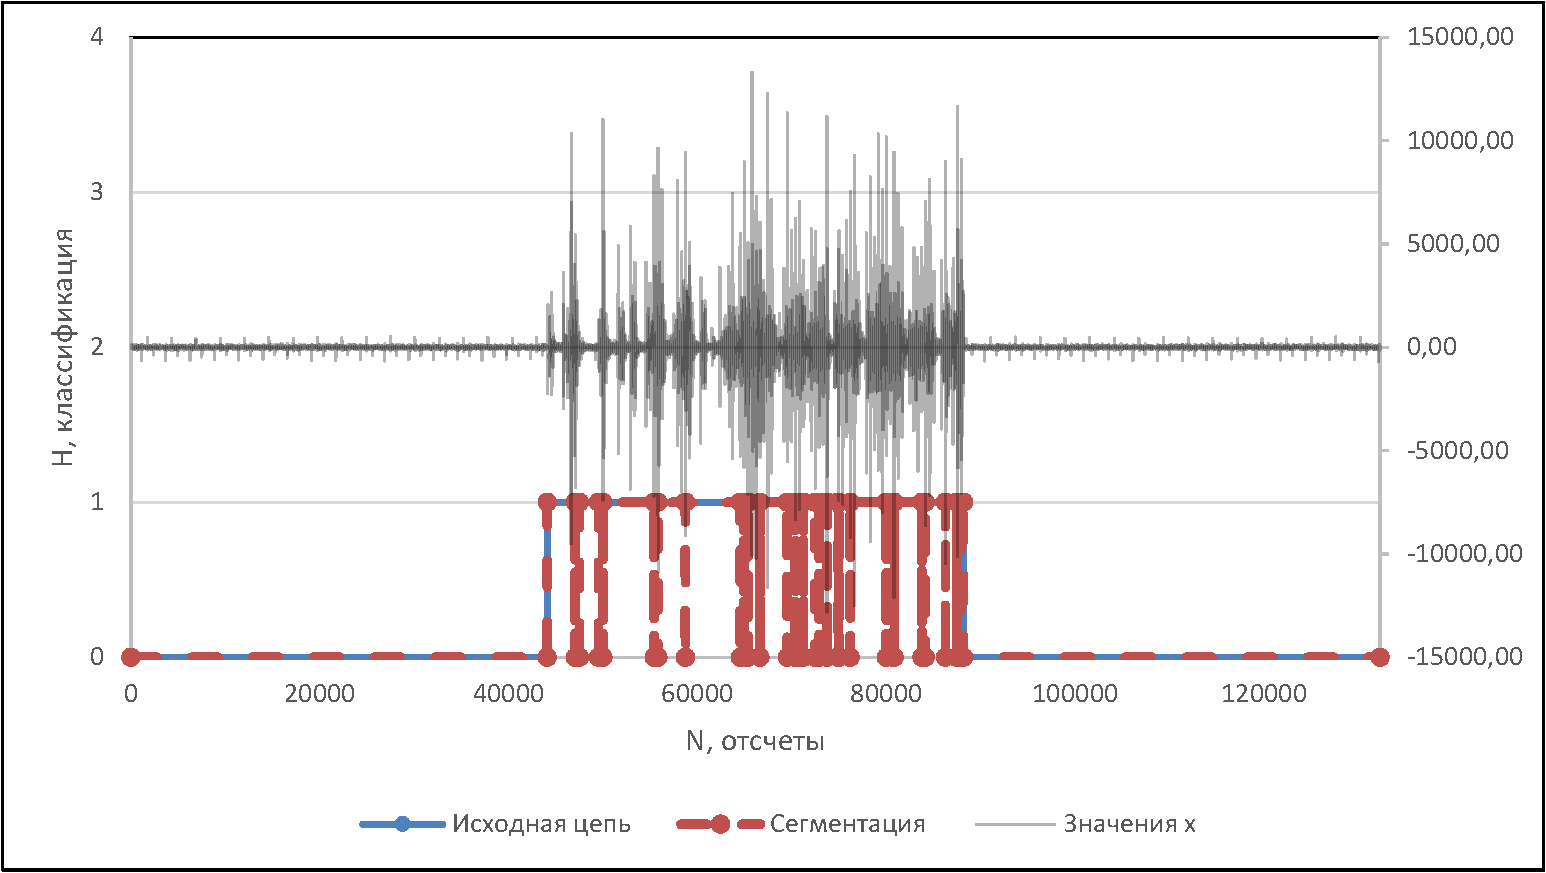
\includegraphics[width=\linewidth]{signal_cropped_2_burobin} \\а)}
\end{minipage}
\begin{minipage}[h]{0.49\linewidth}
\center{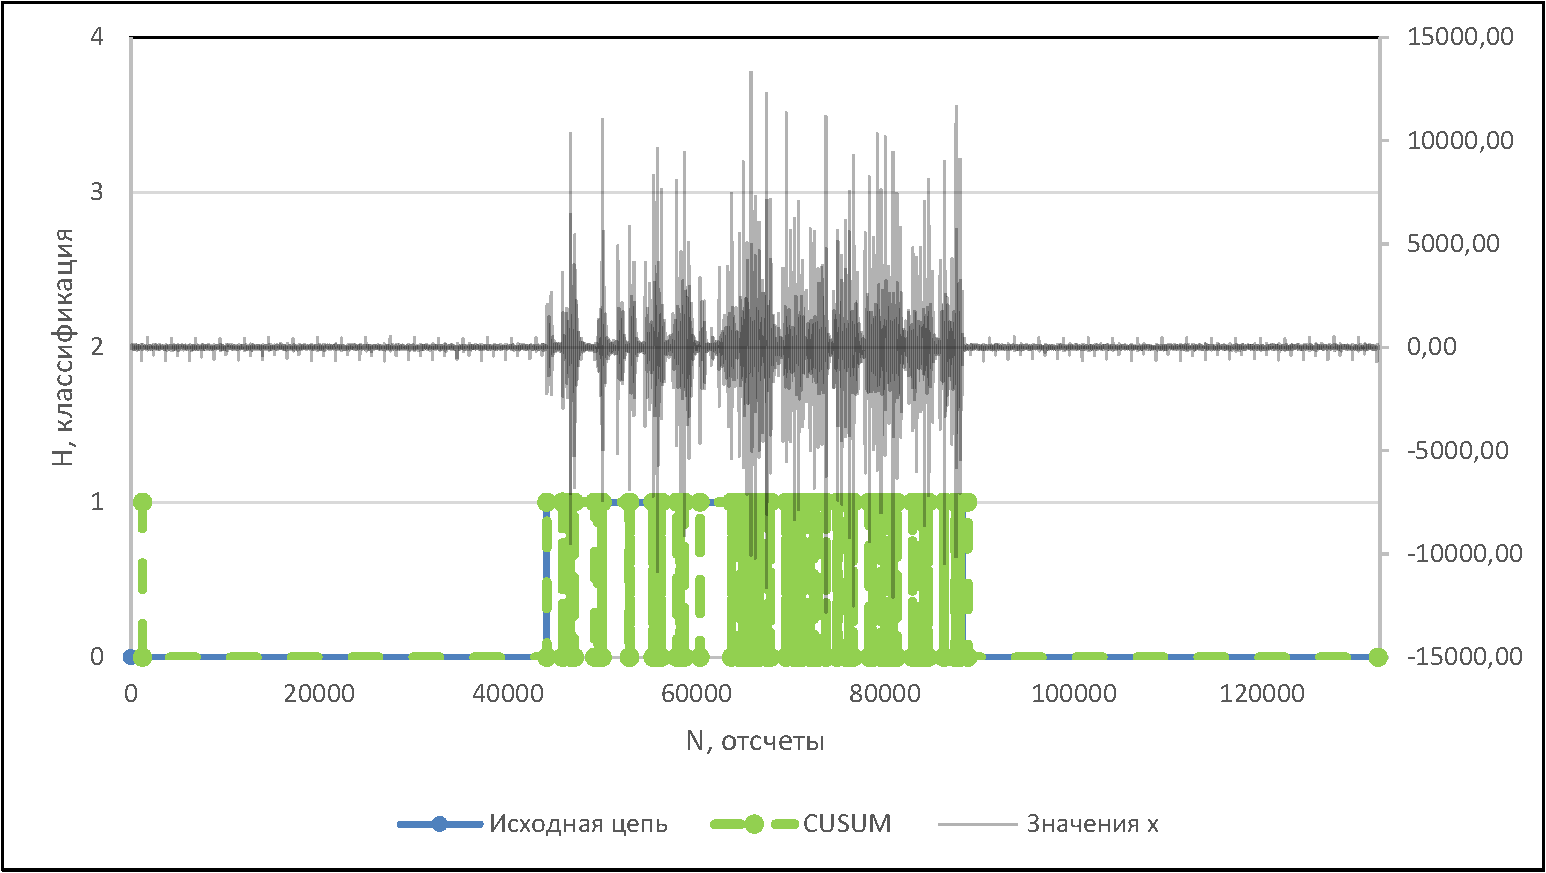
\includegraphics[width=\linewidth]{signal_cropped_2_cusum} \\б)}
\end{minipage}
\caption{Сегментация второго сигнала с вентилятора обоими алгоритмами}
\label{cropped_2}
\end{figure}

\begin{figure}[h!]
\begin{minipage}[h]{0.49\linewidth}
\center{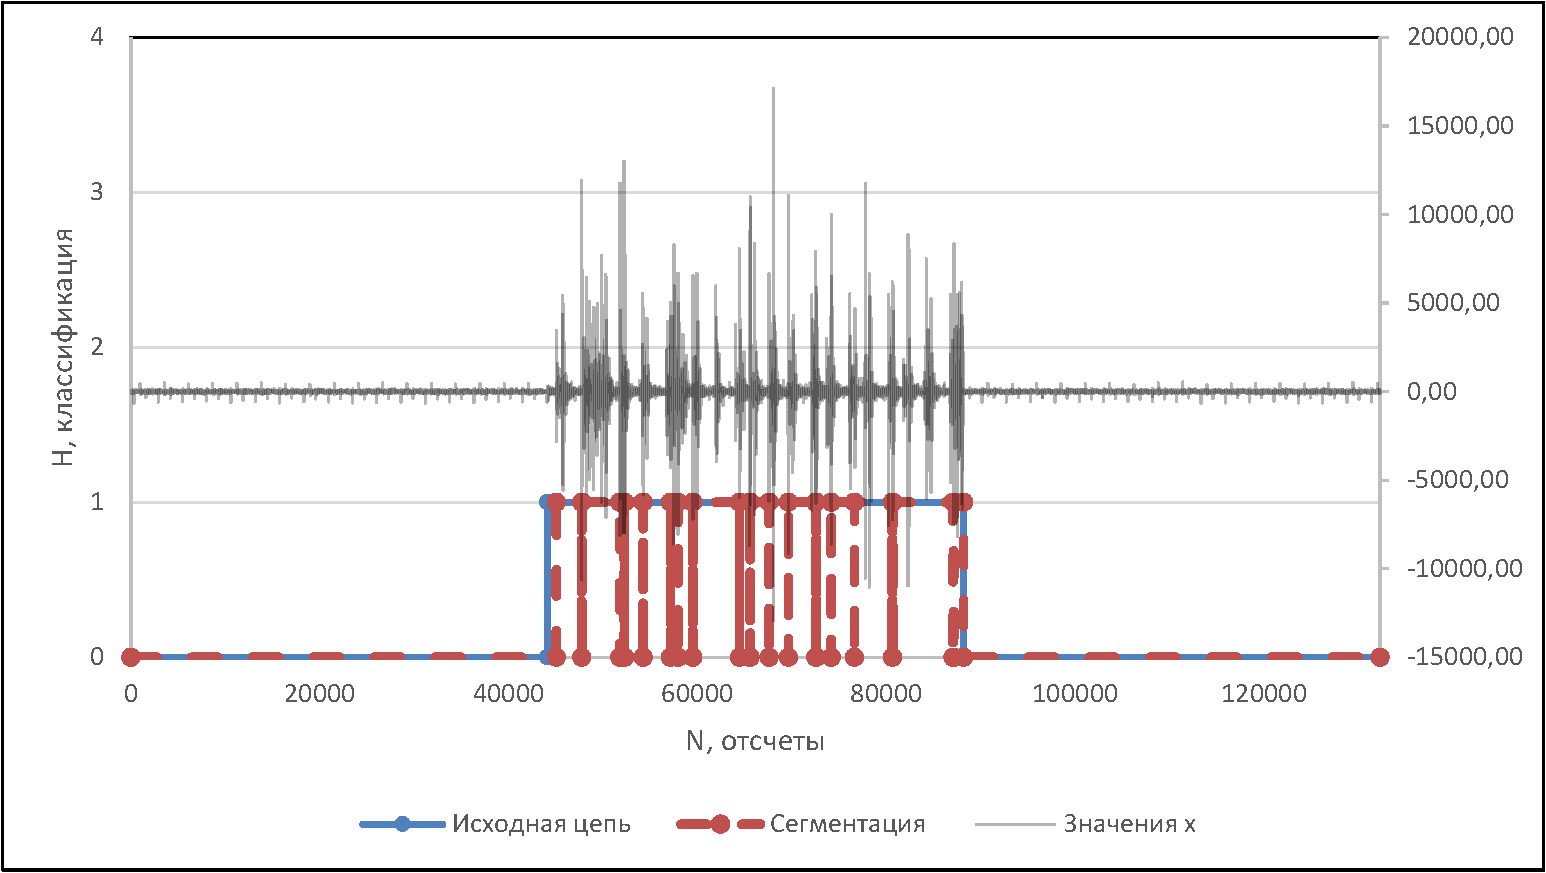
\includegraphics[width=\linewidth]{signal_cropped_3_burobin} \\а)}
\end{minipage}
\begin{minipage}[h]{0.49\linewidth}
\center{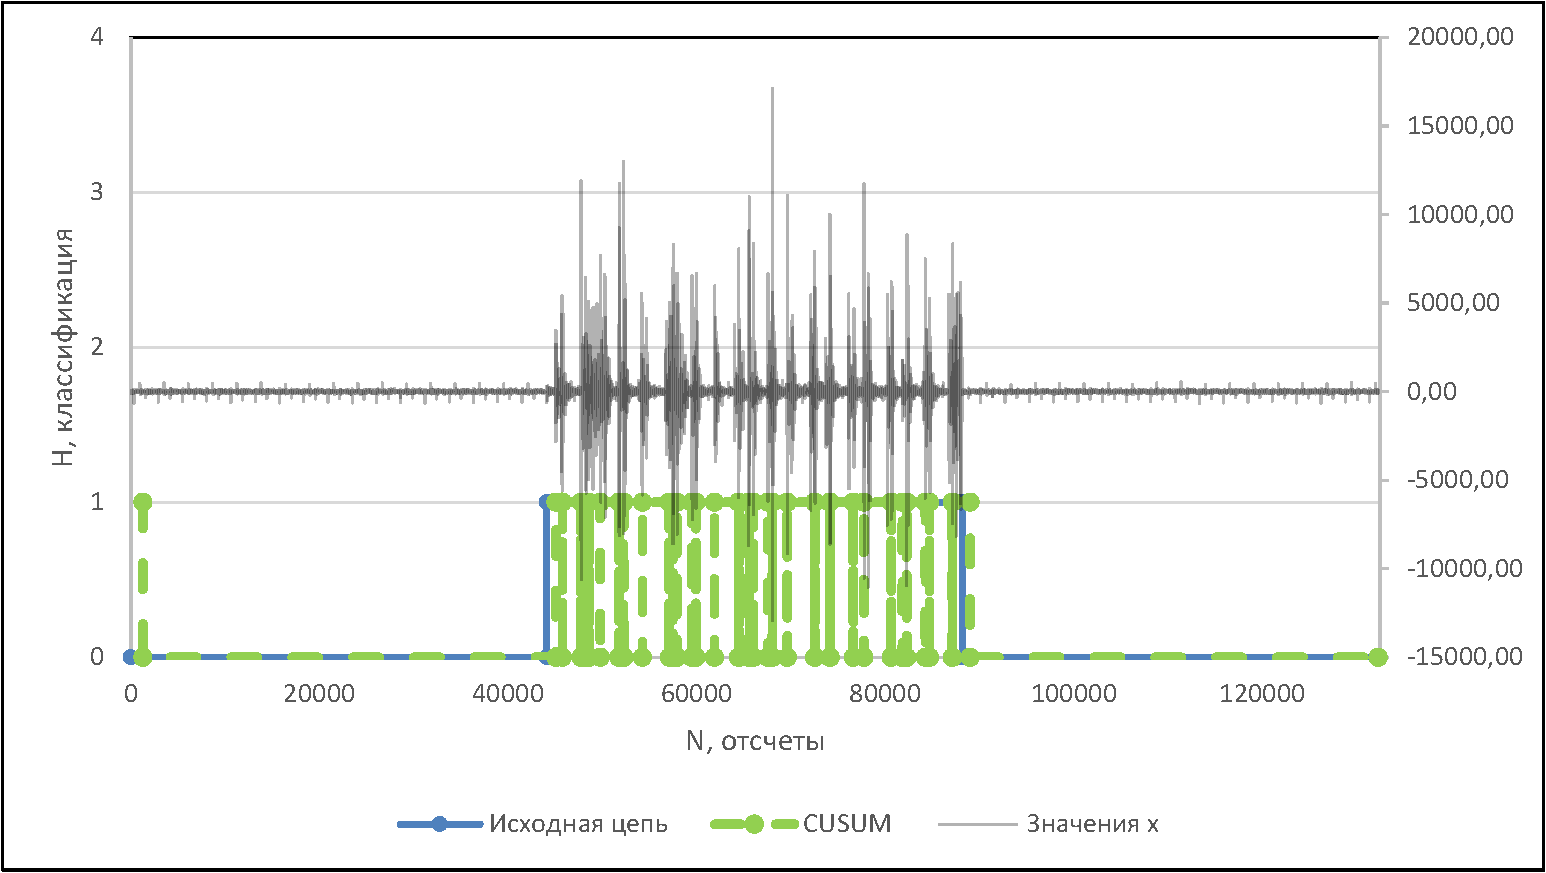
\includegraphics[width=\linewidth]{signal_cropped_3_cusum} \\б)}
\end{minipage}
\caption{Сегментация сигнала 3 с вентилятора обоими алгоритмами}
\label{cropped_3}
\end{figure}

\section{Выводы}
Результаты, полученные из экспериментов с модельным сигналом показывают, что алгоритм\cite{burobin} имеет в среднем на 10 \% большую точность. Это логично, поскольку он учитывает больше данных о входном сигнале, чем CUSUM(а именно вероятности переходов, заданные в матрице $Q$). Алгоритм CUSUM является более легким в реализации и работает быстрее, однако его точность сильно зависит от выбора пороговых значений $T_{ij}$ для каждой пары переходов, что само по себе является довольно неочевидной задачей.

Эксперименты на реальном сигнале с электромеханического устройства(вентилятора) показали, что рассматриваемый подход применим к реальным сигналам, однако требует некоторой доработки.

\addcontentsline{toc}{section}{Литература}
\begin{thebibliography}{99}
\bibitem{TVAR} Chukiet Sodsri, ``Time-varying autoregressive modelling for nonstationary acoustic signal and its frequency analysis'', 2003
\bibitem{vehicles} Kie B. Eom, ``Analysis of Acoustic Signatures from Moving Vehicles Using Time-Varying Autoregressive Models'', Multidimensional Systems and Signal Processing 10, pp. 357-378, 1999
\bibitem{bio} Akay, Y.M., ``Noninvasive acoustical detection of coronary artery disease: a comparative study of signal processing methods'', Biomedical Engineering 40, pp. 571-578, 1993
\bibitem{burobin} Николай Буробин, Вадим Моттль, Илья Мучник, ``Алгоритм определения моментов многократного изменения свойств случайного процесса на основе метода динамического программирования'', Статистические проблемы управления 65, стр. 49-57, 1984.
\bibitem{nikiforov} Mich\`{e}le Basseville, Igor V. Nikiforov, ``Detection of Abrupt Changes: Theory and Application'', pp. 35-43, 1998
\end{thebibliography}
\end{document}